\documentclass[journal,12pt,twocolumn]{IEEEtran}
%
\usepackage{setspace}
\usepackage{gensymb}
%\doublespacing
\singlespacing

%\usepackage{graphicx}
%\usepackage{amssymb}
%\usepackage{relsize}
\usepackage[cmex10]{amsmath}
%\usepackage{amsthm}
%\interdisplaylinepenalty=2500
%\savesymbol{iint}
%\usepackage{txfonts}
%\restoresymbol{TXF}{iint}
%\usepackage{wasysym}
\usepackage{amsthm}
%\usepackage{iithtlc}
\usepackage{mathrsfs}
\usepackage{txfonts}
\usepackage{stfloats}
\usepackage{bm}
\usepackage{cite}
\usepackage{cases}
\usepackage{subfig}
%\usepackage{xtab}
\usepackage{longtable}
\usepackage{multirow}
%\usepackage{algorithm}
%\usepackage{algpseudocode}
\usepackage{enumitem}
\usepackage{mathtools}
\usepackage{steinmetz}
\usepackage{tikz}
\usepackage{circuitikz}
\usepackage{verbatim}
\usepackage{tfrupee}
\usepackage[breaklinks=true]{hyperref}
%\usepackage{stmaryrd}
\usepackage{tkz-euclide} % loads  TikZ and tkz-base
%\usetkzobj{all}
\usetikzlibrary{calc,math}
\usepackage{listings}
    \usepackage{color}                                            %%
    \usepackage{array}                                            %%
    \usepackage{longtable}                                        %%
    \usepackage{calc}                                             %%
    \usepackage{multirow}                                         %%
    \usepackage{hhline}                                           %%
    \usepackage{ifthen}                                           %%
  %optionally (for landscape tables embedded in another document): %%
    \usepackage{lscape}     
\usepackage{multicol}
\usepackage{chngcntr}
%\usepackage{enumerate}

%\usepackage{wasysym}
%\newcounter{MYtempeqncnt}
\DeclareMathOperator*{\Res}{Res}
%\renewcommand{\baselinestretch}{2}
\renewcommand\thesection{\arabic{section}}
\renewcommand\thesubsection{\thesection.\arabic{subsection}}
\renewcommand\thesubsubsection{\thesubsection.\arabic{subsubsection}}

\renewcommand\thesectiondis{\arabic{section}}
\renewcommand\thesubsectiondis{\thesectiondis.\arabic{subsection}}
\renewcommand\thesubsubsectiondis{\thesubsectiondis.\arabic{subsubsection}}

% correct bad hyphenation here
\hyphenation{op-tical net-works semi-conduc-tor}
\def\inputGnumericTable{}                                 %%

\lstset{
%language=C,
frame=single, 
breaklines=true,
columns=fullflexible
}
%\lstset{
%language=tex,
%frame=single, 
%breaklines=true
%}

\begin{document}
%


\newtheorem{theorem}{Theorem}[section]
\newtheorem{problem}{Problem}
\newtheorem{proposition}{Proposition}[section]
\newtheorem{lemma}{Lemma}[section]
\newtheorem{corollary}[theorem]{Corollary}
\newtheorem{example}{Example}[section]
\newtheorem{definition}[problem]{Definition}
%\newtheorem{thm}{Theorem}[section] 
%\newtheorem{defn}[thm]{Definition}
%\newtheorem{algorithm}{Algorithm}[section]
%\newtheorem{cor}{Corollary}
\newcommand{\BEQA}{\begin{eqnarray}}
\newcommand{\EEQA}{\end{eqnarray}}
\newcommand{\define}{\stackrel{\triangle}{=}}

\bibliographystyle{IEEEtran}
%\bibliographystyle{ieeetr}


\providecommand{\mbf}{\mathbf}
\providecommand{\pr}[1]{\ensuremath{\Pr\left(#1\right)}}
\providecommand{\qfunc}[1]{\ensuremath{Q\left(#1\right)}}
\providecommand{\sbrak}[1]{\ensuremath{{}\left[#1\right]}}
\providecommand{\lsbrak}[1]{\ensuremath{{}\left[#1\right.}}
\providecommand{\rsbrak}[1]{\ensuremath{{}\left.#1\right]}}
\providecommand{\brak}[1]{\ensuremath{\left(#1\right)}}
\providecommand{\lbrak}[1]{\ensuremath{\left(#1\right.}}
\providecommand{\rbrak}[1]{\ensuremath{\left.#1\right)}}
\providecommand{\cbrak}[1]{\ensuremath{\left\{#1\right\}}}
\providecommand{\lcbrak}[1]{\ensuremath{\left\{#1\right.}}
\providecommand{\rcbrak}[1]{\ensuremath{\left.#1\right\}}}
\theoremstyle{remark}
\newtheorem{rem}{Remark}
\newcommand{\sgn}{\mathop{\mathrm{sgn}}}
\providecommand{\abs}[1]{\left\vert#1\right\vert}
\providecommand{\res}[1]{\Res\displaylimits_{#1}} 
\providecommand{\norm}[1]{\left\lVert#1\right\rVert}
%\providecommand{\norm}[1]{\lVert#1\rVert}
\providecommand{\mtx}[1]{\mathbf{#1}}
\providecommand{\mean}[1]{E\left[ #1 \right]}
\providecommand{\fourier}{\overset{\mathcal{F}}{ \rightleftharpoons}}
%\providecommand{\hilbert}{\overset{\mathcal{H}}{ \rightleftharpoons}}
\providecommand{\system}{\overset{\mathcal{H}}{ \longleftrightarrow}}
	%\newcommand{\solution}[2]{\textbf{Solution:}{#1}}
\newcommand{\solution}{\noindent \textbf{Solution: }}
\newcommand{\cosec}{\,\text{cosec}\,}
\providecommand{\dec}[2]{\ensuremath{\overset{#1}{\underset{#2}{\gtrless}}}}
\newcommand{\myvec}[1]{\ensuremath{\begin{pmatrix}#1\end{pmatrix}}}
\newcommand{\mydet}[1]{\ensuremath{\begin{vmatrix}#1\end{vmatrix}}}
%\numberwithin{equation}{section}
\numberwithin{equation}{subsection}
%\numberwithin{problem}{section}
%\numberwithin{definition}{section}
\makeatletter
\@addtoreset{figure}{problem}
\makeatother

\let\StandardTheFigure\thefigure
\let\vec\mathbf
%\renewcommand{\thefigure}{\theproblem.\arabic{figure}}
\renewcommand{\thefigure}{\theproblem}
%\setlist[enumerate,1]{before=\renewcommand\theequation{\theenumi.\arabic{equation}}
%\counterwithin{equation}{enumi}


%\renewcommand{\theequation}{\arabic{subsection}.\arabic{equation}}

\def\putbox#1#2#3{\makebox[0in][l]{\makebox[#1][l]{}\raisebox{\baselineskip}[0in][0in]{\raisebox{#2}[0in][0in]{#3}}}}
     \def\rightbox#1{\makebox[0in][r]{#1}}
     \def\centbox#1{\makebox[0in]{#1}}
     \def\topbox#1{\raisebox{-\baselineskip}[0in][0in]{#1}}
     \def\midbox#1{\raisebox{-0.5\baselineskip}[0in][0in]{#1}}

\vspace{3cm}


\title{Que: 11.11.4.9}
\author{Nikam Pratik Balasaheb (EE21BTECH11037)}





% make the title area
\maketitle

\newpage

%\tableofcontents

\bigskip

\renewcommand{\thefigure}{\theenumi}
\renewcommand{\thetable}{\theenumi}
%\renewcommand{\theequation}{\theenumi}

\section{Problem}
Find the equations of hyperbola having Vertices $\myvec{0\\\pm 3}$ and Foci $\myvec{0\\\pm5}$

\section{Solution}

\begin{enumerate}

	\item Transverse axis:
Line joining two foci
\begin{align}
	\vec{m} &= \vec{F}_1 - \vec{F}_2\\
	&= \myvec{0 \\ 10}\\
	\myvec{1&0}\brak{\vec{x} -\vec{F}_1} &= 0\\
	\myvec{1& 0}\vec{x} &= 0
\end{align}

\item Center of hyperbola, $\vec{O}$ is given by:
\begin{align}
	\vec{O} &= \frac{\vec{F}_1 + \vec{F}_2}{2}\\
	\vec{O} &= \myvec{0\\0}
\end{align}

\item Normal vector of directrix
	\begin{align}
		\vec{n} &= \text{direction vector of transverse axis}\\
			&= \myvec{0 \\1}
	\end{align}

\begin{align}
	\vec{V} &= \norm{\vec{n}}^2\vec{I} - e^2\vec{n}\vec{n}^{\top}\\
		&= \myvec{1 & 0 \\ 0 & 1} - e^2\myvec{ 0 & 0 \\ 0 & 1}\\
		&= \myvec{1 &0\\ 0 & 1-e^2}
\end{align}

\begin{align}
	\vec{u} &= ce^2\vec{n} -\norm{\vec{n}}^2\vec{F}\\
		&= \myvec{0\\ ce^2 - 5}
\end{align}

\begin{align}
	f &= \norm{\vec{n}}^2\norm{\vec{F}}^2 - c^2e^2\\
	  &= 25 - c^2 e^2
\end{align}

Equation of the hyperbola:
\begin{align}
	\vec{x}^{\top}\vec{V}\vec{x} +2\vec{u}^{\top}\vec{x}+f &= 0\\
\end{align}

Vertex lies on this curve,
\begin{align}
	\vec{v_1}^{\top}\vec{V}\vec{v_1} +2\vec{u}^{\top}\vec{v_1}+f &= 0\\
	9\brak{1-e^2} + 6 \brak{ce^2 -5} - c^2e^2 +25 &= 0\\
	4 -9e^2 +6ce^2 -c^2e^2 &= 0 \label{eq:1}
\end{align}
Also, the center is given by,
\begin{align}
	\vec{O} &= - \vec{V}^{-1} \vec{u}\\
	\myvec{0\\0} &= \myvec{0\\ \frac{ce^2-5}{1-e^2}}\\
	ce^2 &= 5
	\label{eq:2}
\end{align}

Solving \eqref{eq:1} and \eqref{eq:2},
\begin{align}
	c &= \frac{9}{5} \\
	e &= \frac{5}{3}\\
\end{align}

\begin{align}
	\vec{V} &= \myvec{1&0\\0& -\frac{16}{9}} \\
	\vec{u} &= \myvec{0\\0}\\
	f &= 16\\
\end{align}

Equation of the Hyperbola,
\begin{align}
	\vec{x}^{\top} \myvec{1&0\\ 0 & -\frac{16}{9}} \vec{x} +16 =0
\end{align}

\begin{table}[h!]
	\begin{center}
	%%%%%%%%%%%%%%%%%%%%%%%%%%%%%%%%%%%%%%%%%%%%%%%%%%%%%%%%%%%%%%%%%%%%%%
%%                                                                  %%
%%  This is a LaTeX2e table fragment exported from Gnumeric.        %%
%%                                                                  %%
%%%%%%%%%%%%%%%%%%%%%%%%%%%%%%%%%%%%%%%%%%%%%%%%%%%%%%%%%%%%%%%%%%%%%%

\begin{tabular}[]{|c|c|c|}
\hline
$\vec{O}$	& $\myvec{5\\0}$ &Center of the given circle \\ \hline
$\vec{B}$	& $\myvec{0\\0}$ &Point where Salma is standing\\ \hline
$r$		& 5 & radius of given circle \\ \hline
$d$ 		& 6 & distance AB and BC\\ \hline
\end{tabular}

\end{center}
\caption{Table1}
\label{tab:}
\end{table}

\begin{figure}[h!]
  \centering
    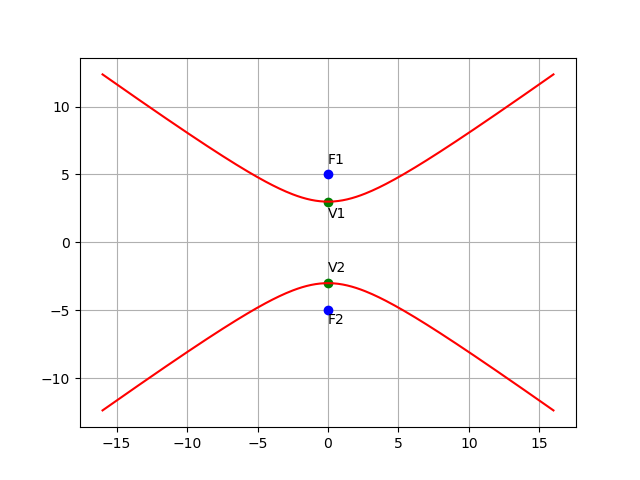
\includegraphics[width=\columnwidth]{figs/Figure_1.png}
    \caption{Figure 1}
    \label{fig:}
\end{figure}

\end{enumerate}
\end{document}



